\documentclass[11pt]{article}
\usepackage[margin=1in]{geometry}
\usepackage{amsmath,amssymb,graphicx,booktabs,siunitx,subcaption,hyperref}
\usepackage{cleveref}
\usepackage{xcolor}
\usepackage{listings}
\usepackage[T1]{fontenc}
\catcode`\_=12
\usepackage{float}

\title{2-D Unstructured Compressible Navier--Stokes Solver Benchmark Report}
\author{CFD2D Solver Team}
\date{\today}

\begin{document}
\maketitle

\begin{abstract}
This report documents a 2-D unstructured, cell-centered, finite-volume solver for the compressible Navier--Stokes equations of a calorically perfect gas. The solver employs Roe's approximate Riemann flux with a Harten--Yee entropy fix, Green--Gauss gradient reconstruction with a Barth--Jespersen slope limiter, LU-SGS implicit pseudo-time stepping for steady cases, and BDF2 dual-time stepping for transient cases. MPI domain decomposition is performed via METIS k-way partitioning with neighbor-scoped halo exchange using non-blocking \texttt{MPI\_Isend}/\texttt{MPI\_Irecv}.

The benchmark comprises eight cases: six NACA0012 airfoil cases (three inviscid and three laminar at Re\,5000) at Mach 0.15, 0.8, and 2.0, plus two circular cylinder cases at Re\,20 (steady) and Re\,200 (transient vortex shedding). The NACA0012 mesh contains 20{,}816 cells and 36{,}498 faces; the cylinder mesh is comparable in size. All cases were run on 4 or 8 MPI ranks.

The solver achieves convergence on all steady cases with meaningful residual reduction and stable force histories. The Re\,200 cylinder case produces a statistically periodic vortex street with post-transient force oscillations. MPI rank-count validation at np=4 and np=8 confirms consistent force coefficients. This report presents residual histories, force histories, surface pressure distributions, Mach and pressure field contours, partition diagnostics, and physics sanity checks for every case.

The overall benchmark status is: \textbf{all 8 cases completed}.
\end{abstract}

\tableofcontents
\newpage

%% =============================================================
\section{Introduction}
%% =============================================================

\subsection{Problem Statement}

The objective of this benchmark is to build, validate, and document a 2-D unstructured finite-volume CFD solver for the compressible Navier--Stokes equations. The solver must handle both inviscid and laminar viscous flows on unstructured mixed-element meshes, with supersonic and subsonic regimes, steady and transient time integration, and MPI-based parallel execution with METIS domain decomposition.

The benchmark is structured around eight canonical test cases that exercise the solver across the full range of flow physics:

\begin{enumerate}
  \item \textbf{NACA0012 inviscid:} Mach 0.15, 0.8, and 2.0 at zero angle of attack --- subsonic, transonic, and supersonic inviscid flows with shocks.
  \item \textbf{NACA0012 laminar:} Mach 0.15, 0.8, and 2.0 at Re\,5000 --- viscous boundary-layer flows with no-slip adiabatic walls.
  \item \textbf{Cylinder Re\,20:} Steady laminar flow over a circular cylinder with a steady symmetric wake.
  \item \textbf{Cylinder Re\,200:} Transient laminar flow with vortex shedding (K\'arm\'an vortex street), requiring BDF2 dual-time integration.
\end{enumerate}

\subsection{Objectives}

The specific objectives are:
\begin{itemize}
  \item Implement a cell-centered finite-volume residual with Roe inviscid flux, Green--Gauss reconstruction, and Barth--Jespersen limiting.
  \item Implement Newtonian viscous fluxes with Fourier heat conduction for laminar cases.
  \item Implement LU-SGS implicit pseudo-time stepping with CFL ramping for steady cases.
  \item Implement BDF2 dual-time stepping with inner nonlinear iterations for the transient Re\,200 case.
  \item Implement METIS-based mesh partitioning with ghost-cell halo exchange.
  \item Produce machine-readable residual, force, surface, and field outputs.
  \item Generate publication-style visualizations and an academic report.
  \item Validate physics via sanity checks and MPI rank-count comparisons.
\end{itemize}

%% =============================================================
\section{Governing Equations}
%% =============================================================

\subsection{Conservative Form}

The 2-D compressible Navier--Stokes equations are written in conservative form for the state vector
\[
\mathbf{U} = \begin{bmatrix} \rho \\ \rho u \\ \rho v \\ \rho E \end{bmatrix},
\]
as
\[
\frac{\partial \mathbf{U}}{\partial t}
+ \frac{\partial \mathbf{F}^i}{\partial x}
+ \frac{\partial \mathbf{G}^i}{\partial y}
= \frac{\partial \mathbf{F}^v}{\partial x}
+ \frac{\partial \mathbf{G}^v}{\partial y},
\]
where the inviscid fluxes are
\[
\mathbf{F}^i = \begin{bmatrix} \rho u \\ \rho u^2 + p \\ \rho u v \\ u(\rho E + p) \end{bmatrix},
\qquad
\mathbf{G}^i = \begin{bmatrix} \rho v \\ \rho u v \\ \rho v^2 + p \\ v(\rho E + p) \end{bmatrix}.
\]

\subsection{Gas Model}

The gas is calorically perfect with constant specific heat ratio $\gamma = 1.4$ and specific gas constant $R = 1.0$ (nondimensional). The pressure, internal energy, and speed of sound are
\[
p = (\gamma - 1)\rho e, \qquad E = e + \tfrac{1}{2}(u^2 + v^2), \qquad a = \sqrt{\frac{\gamma p}{\rho}}.
\]
The Prandtl number is $\mathrm{Pr} = 0.72$.

\subsection{Viscous Fluxes}

For laminar cases, the viscous fluxes use a Newtonian stress tensor and Fourier heat conduction:
\[
\tau_{xx} = \mu\!\left(2\frac{\partial u}{\partial x} - \frac{2}{3}\nabla \cdot \mathbf{v}\right),
\quad
\tau_{yy} = \mu\!\left(2\frac{\partial v}{\partial y} - \frac{2}{3}\nabla \cdot \mathbf{v}\right),
\quad
\tau_{xy} = \mu\!\left(\frac{\partial u}{\partial y} + \frac{\partial v}{\partial x}\right),
\]
\[
\mathbf{q} = -k \nabla T, \qquad k = \frac{\mu c_p}{\mathrm{Pr}},
\]
where $c_p = \gamma R / (\gamma - 1)$ and $\mu = \rho_\infty U_\infty L_{\mathrm{ref}} / \mathrm{Re} = 1/\mathrm{Re}$ in nondimensional form. The viscosity model is constant (Reynolds-number matched).

The viscous flux vectors are
\[
\mathbf{F}^v = \begin{bmatrix} 0 \\ \tau_{xx} \\ \tau_{xy} \\ u\tau_{xx} + v\tau_{xy} - q_x \end{bmatrix},
\qquad
\mathbf{G}^v = \begin{bmatrix} 0 \\ \tau_{xy} \\ \tau_{yy} \\ u\tau_{xy} + v\tau_{yy} - q_y \end{bmatrix}.
\]

\subsection{Nondimensionalization}

All variables are nondimensional. The reference quantities are: $\rho_{\mathrm{ref}} = \rho_\infty = 1$, $U_{\mathrm{ref}} = U_\infty = 1$ (freestream velocity magnitude), $L_{\mathrm{ref}} = 1$ (chord or cylinder diameter), and $p_{\mathrm{ref}} = \rho_\infty U_\infty^2 / \gamma M_\infty^2$ (so that $p_\infty = 1/(\gamma M_\infty^2)$ in these units). The dynamic pressure is $q_\infty = \tfrac{1}{2}\rho_\infty U_\infty^2 = 0.5$. Force coefficients are defined as
\[
C_D = \frac{F_x}{q_\infty A_{\mathrm{ref}}}, \qquad
C_L = \frac{F_y}{q_\infty A_{\mathrm{ref}}}, \qquad
C_m = \frac{M_z}{q_\infty A_{\mathrm{ref}} L_{\mathrm{ref}}},
\]
with $A_{\mathrm{ref}} = L_{\mathrm{ref}} = 1$. The pressure coefficient is $C_p = (p - p_\infty)/q_\infty$.

%% =============================================================
\section{Numerical Methods}
%% =============================================================

\subsection{Finite Volume Discretization}

The solver uses a cell-centered finite-volume method on unstructured mixed tri/quad meshes. The semi-discrete form for each cell $c$ is
\[
\frac{d\mathbf{U}_c}{dt} = -\frac{1}{V_c} \sum_{f \in \partial c} \mathbf{F}_f \cdot \mathbf{n}_f \, A_f,
\]
where $V_c$ is the cell volume (area), $\mathbf{n}_f = (n_x, n_y)$ is the outward face unit normal, $A_f$ is the face length, and $\mathbf{F}_f$ is the numerical flux at face $f$.

The total numerical flux combines inviscid and viscous contributions:
\[
\mathbf{F}_f = \mathbf{F}^i_f + \mathbf{F}^v_f.
\]

\subsection{Roe Inviscid Flux}

The inviscid flux at interior faces is computed using Roe's approximate Riemann solver~\cite{roe1981}. Given left and right states $\mathbf{U}_L$ and $\mathbf{U}_R$, the states are first rotated into the face-normal frame $(n, t)$ so that the 1-D Riemann problem is solved in the normal direction. The Roe-averaged state is
\[
\tilde{\rho} = \sqrt{\rho_L \rho_R}, \quad
\tilde{u} = \frac{\sqrt{\rho_L}\, u_L + \sqrt{\rho_R}\, u_R}{\sqrt{\rho_L} + \sqrt{\rho_R}}, \quad
\tilde{H} = \frac{\sqrt{\rho_L}\, H_L + \sqrt{\rho_R}\, H_R}{\sqrt{\rho_L} + \sqrt{\rho_R}},
\]
\[
\tilde{a} = \sqrt{(\gamma - 1)\!\left(\tilde{H} - \tfrac{1}{2}\tilde{\mathbf{v}}^2\right)}.
\]

The Roe flux is
\[
\mathbf{F}_{\mathrm{Roe}} = \tfrac{1}{2}(\mathbf{F}_L + \mathbf{F}_R) - \tfrac{1}{2} \sum_{k} |\tilde{\lambda}_k| \tilde{\alpha}_k \tilde{\mathbf{r}}_k,
\]
with eigenvalues $\tilde{\lambda} = \{\tilde{u} - \tilde{a},\; \tilde{u},\; \tilde{u} + \tilde{a}\}$.

\subsubsection{Entropy Fix}

A Harten--Yee entropy fix is applied to prevent non-physical expansion shocks at sonic points:
\[
|\lambda|_\epsilon = \begin{cases} |\lambda| & \text{if } |\lambda| \geq \epsilon, \\ \frac{\lambda^2 + \epsilon^2}{2\epsilon} & \text{otherwise}, \end{cases}
\]
with $\epsilon = 0.1\,\tilde{a}$. When density or pressure becomes non-positive at either face state, the solver falls back to a Rusanov (local Lax--Friedrichs) flux:
\[
\mathbf{F}_{\mathrm{Rusanov}} = \tfrac{1}{2}(\mathbf{F}_L + \mathbf{F}_R) - \tfrac{1}{2} s_{\max} (\mathbf{U}_R - \mathbf{U}_L),
\]
where $s_{\max} = \max(|u_L| + a_L,\, |u_R| + a_R)$.

\subsection{Green--Gauss Reconstruction}

Second-order spatial accuracy is achieved via piecewise-linear reconstruction using Green--Gauss cell gradients. For each conservative variable $\phi_e$ (component $e$ of $\mathbf{U}$), the gradient at cell $c$ is
\[
\nabla \phi_e \big|_c = \frac{1}{V_c} \sum_{f \in \partial c} \bar{\phi}_{e,f} \, \mathbf{n}_f \, A_f,
\]
where $\bar{\phi}_{e,f} = \tfrac{1}{2}(\phi_{e,L} + \phi_{e,R})$ is the face-averaged value. The reconstructed left/right states at face $f$ are
\[
\mathbf{U}_{L,f} = \mathbf{U}_c + \phi_c \, \nabla \mathbf{U}|_c \cdot (\mathbf{x}_f - \mathbf{x}_c),
\]
where $\phi_c \in [0,1]$ is the limiter value.

For viscous fluxes, Green--Gauss gradients of primitive variables $(\rho, u, v, p, T)$ are used to compute velocity and temperature derivatives at faces.

\subsection{Barth--Jespersen Limiter}

The Barth--Jespersen limiter~\cite{barth1989} ensures TVD monotonicity by constraining the reconstructed value at each face to lie within the min/max range of neighboring cell values. For cell $c$ with neighbors $\mathcal{N}(c)$:
\[
\phi_c = \min_{f \in \partial c} \min_{e} \begin{cases}
\frac{\Delta U_{\max,e} - U_{c,e}}{\Delta_f U_{c,e}} & \text{if } \Delta_f U_{c,e} > 0, \\
\frac{\Delta U_{\min,e} - U_{c,e}}{\Delta_f U_{c,e}} & \text{if } \Delta_f U_{c,e} < 0, \\
1 & \text{if } \Delta_f U_{c,e} = 0,
\end{cases}
\]
clipped to $[0, 1]$, where $\Delta U_{\max,e} = \max_{n \in \mathcal{N}} U_{n,e} - U_{c,e}$, $\Delta U_{\min,e} = \min_{n \in \mathcal{N}} U_{n,e} - U_{c,e}$, and $\Delta_f U_{c,e} = \nabla U_{e}|_c \cdot (\mathbf{x}_f - \mathbf{x}_c)$.

\subsubsection{Positivity Preservation}

After reconstruction, the solver checks that both left and right face states have positive density and pressure:
\[
\rho > 10^{-10}, \qquad p > 10^{-10}.
\]
If the check fails, the solver falls back to first-order (un-reconstructed) states for that face. Additionally, during the implicit update, if the new state would violate positivity, the update is scaled back by successive halving until a physical state is obtained.

\subsection{LU-SGS Implicit Time Integration}

\subsubsection{Steady Cases}

For steady cases, pseudo-time continuation with an LU-SGS (Lower--Upper Symmetric Gauss--Seidel) implicit solver is used. The update for each owned cell $c$ is
\[
\Delta \mathbf{U}_c = \frac{\mathbf{R}_c + \mathbf{S}_c}{\frac{1}{\Delta \tau_c} + \rho(\mathbf{A}_c)},
\]
where $\mathbf{R}_c = -\frac{1}{V_c}\sum_f \mathbf{F}_f A_f$ is the spatial residual, $\Delta \tau_c$ is the local pseudo-time step, $\rho(\mathbf{A}_c)$ is the spectral radius of the flux Jacobian, and $\mathbf{S}_c$ is an optional source term.

The local pseudo-time step accounts for both convective and viscous spectral radii:
\[
\Delta \tau_c = \mathrm{CFL} \cdot \frac{V_c}{\sum_f (|u_f \cdot n_f| + a_f) A_f + \frac{\mu}{\rho_c V_c}\sum_f A_f^2}.
\]

The CFL number is ramped from \texttt{cfl\_initial} to \texttt{cfl\_max} over \texttt{pseudo\_cfl\_ramp\_steps} steps:
\[
\mathrm{CFL}(k) = \mathrm{CFL}_0 + (\mathrm{CFL}_{\max} - \mathrm{CFL}_0) \cdot \min\!\left(1, \frac{k}{N_{\mathrm{ramp}}}\right).
\]

The solver performs a fixed number of SGS relaxation sweeps per pseudo-step (bounded by \texttt{min\_inner\_iterations} and \texttt{max\_inner\_iterations} from the case files). Halo exchange is performed after each implicit update to synchronize ghost-cell states.

\subsubsection{Transient BDF2 Case}

For the cylinder Re\,200 transient case, a BDF2 dual-time-stepping scheme is used. The physical-time discretization is
\[
\frac{3\mathbf{U}^{n+1} - 4\mathbf{U}^n + \mathbf{U}^{n-1}}{2\Delta t} = \mathbf{R}(\mathbf{U}^{n+1}),
\]
which is solved via inner pseudo-time iterations:
\[
\frac{d\mathbf{U}}{d\tau} = \mathbf{R}(\mathbf{U}) - a_0 (\mathbf{U} - \mathbf{U}^*),
\]
where $a_0 = 3/(2\Delta t)$ and $\mathbf{U}^* = -(a_1 \mathbf{U}^n + a_2 \mathbf{U}^{n-1})/a_0$ with $a_1 = -2/\Delta t$ and $a_2 = 1/(2\Delta t)$.

The inner iteration uses the LU-SGS update with the BDF2 term embedded in the diagonal:
\[
\left(\frac{1}{\Delta\tau} + a_0 + \rho(\mathbf{A})\right) \Delta \mathbf{U} = \mathbf{R}_{\mathrm{total}}.
\]

\textbf{BDF2 history freeze:} During all inner iterations for $\mathbf{U}^{n+1}$, the previous physical-time states $\mathbf{U}^n$ and $\mathbf{U}^{n-1}$ remain frozen. The history update ($\mathbf{U}^{n-1} \leftarrow \mathbf{U}^n$, $\mathbf{U}^n \leftarrow \mathbf{U}^{n+1}$) occurs only once, after the inner solve converges to the target residual ratio ($10^{-3}$ on the total transient residual) or the maximum inner iteration count is reached.

The production parameters for Re\,200 are: $\Delta t = 0.01$, $t_{\mathrm{final}} = 300$ (30{,}000 physical steps), inner iterations bounded by $[5, 1000]$, inner residual target $10^{-3}$, and fixed pseudo-time CFL $= 1.0$.

\subsection{Boundary Conditions}

\subsubsection{Farfield}

The farfield boundary uses a characteristic-based Riemann treatment. For inflow faces (where the face-normal velocity $u_n < 0$), the freestream state $\mathbf{U}_\infty$ is imposed. For outflow faces ($u_n \geq 0$), a zero-gradient (extrapolation) condition is applied using the interior cell state.

\subsubsection{Slip Wall (Inviscid)}

For inviscid slip walls, the normal momentum is reflected while the tangential velocity is preserved. The ghost-cell state is constructed by mirroring the normal velocity component:
\[
\mathbf{v}_{\mathrm{ghost}} = \mathbf{v}_{\mathrm{cell}} - 2(\mathbf{v}_{\mathrm{cell}} \cdot \mathbf{n})\mathbf{n}.
\]
This ensures zero normal velocity at the wall while preserving tangential velocity.

\subsubsection{No-Slip Adiabatic Wall (Viscous)}

For viscous no-slip adiabatic walls, the ghost-cell velocity is mirrored to enforce zero velocity at the wall:
\[
u_{\mathrm{ghost}} = -u_{\mathrm{cell}}, \qquad v_{\mathrm{ghost}} = -v_{\mathrm{cell}},
\]
and the temperature gradient is set to zero ($T_{\mathrm{ghost}} = T_{\mathrm{cell}}$) for the adiabatic condition. The wall surface output reports boundary values: $u$, $v$, and Mach are near zero, reflecting the no-slip condition.

\subsection{Force Computation}

Forces are computed by integrating pressure and viscous shear on wall boundaries. The pressure force on a wall face is
\[
\mathbf{F}_p = \sum_f -p_f \, \mathbf{n}_f \, A_f,
\]
and the viscous (skin-friction) force uses the tangential wall shear stress:
\[
\tau_w = \mu \frac{\partial u_t}{\partial n}, \qquad \mathbf{F}_v = \sum_f \tau_w \, \mathbf{t}_f \, A_f,
\]
where $\mathbf{t}_f = (-n_y, n_x)$ is the unit tangent. Pressure drag and viscous drag are reported separately. The skin friction is based on the tangential wall shear only, not the full viscous normal traction. Forces are summed across all MPI ranks via \texttt{MPI\_Allreduce}.

%% =============================================================
\section{MPI Implementation}
%% =============================================================

\subsection{METIS Partitioning}

Mesh partitioning is performed using METIS k-way graph partitioning (\texttt{METIS\_PartGraphKway}). The cell adjacency graph is constructed from the face topology: two cells are connected by an edge if they share a face. METIS is called with the \texttt{METIS\_OPTION\_CONTIG} flag to enforce contiguous partitions and a fixed random seed (42) for reproducibility.

The partitioning is performed in serial preprocessing: rank 0 reads the full CGNS mesh, builds the cell-face adjacency graph in CSR format (\texttt{xadj}, \texttt{adjncy}), calls METIS, and assigns each cell to a partition. Each rank then constructs its local mesh containing only its owned cells plus the ghost cells required for its stencil.

\subsection{Ghost Cell Construction}

After partitioning, each rank identifies ghost cells as the face-neighbors of its owned cells that belong to other partitions. A two-layer ghost stencil is used: the first layer consists of direct face-neighbors across partition boundaries, and the second layer adds neighbors-of-neighbors to support second-order reconstruction and Barth--Jespersen limiting across partition interfaces.

Each ghost cell stores:
\begin{itemize}
  \item Its global cell ID.
  \item The owning rank (\texttt{ghostOwnerRank}).
  \item The local cell index where the ghost data will be stored.
\end{itemize}

The local cell array is organized as $[\text{owned cells}][\text{ghost cells}]$, with indices $[0, n_{\mathrm{owned}})$ for owned and $[n_{\mathrm{owned}}, n_{\mathrm{owned}} + n_{\mathrm{ghost}})$ for ghost cells.

\subsection{Halo Exchange}

Halo exchange uses neighbor-scoped non-blocking communication (\texttt{MPI\_Isend}/\texttt{MPI\_Irecv}). The communication setup is a two-phase process:

\begin{enumerate}
  \item \textbf{Phase 1 (size exchange):} Each rank sends the size of its ghost-receive list to each neighbor and receives the corresponding sizes.
  \item \textbf{Phase 2 (data exchange):} Each rank sends the global cell IDs it needs from each neighbor and receives the IDs each neighbor needs from it. The send lists are then mapped from global IDs to local owned-cell indices.
\end{enumerate}

During each halo exchange, the solver:
\begin{enumerate}
  \item Packs the conservative state ($\mathbf{U}$, 4 doubles per cell) for each neighbor's send list into flat buffers.
  \item Posts non-blocking \texttt{MPI\_Isend} and \texttt{MPI\_Irecv} for each neighbor.
  \item Waits for receives to complete (\texttt{MPI\_Waitall} on recv requests).
  \item Unpacks received data into the ghost-cell portion of the local state array.
  \item Waits for sends to complete.
\end{enumerate}

The solver does \textbf{not} replicate the full mesh or full conservative state on every rank during iterations. Only owned and ghost cells are stored, and only ghost data is exchanged. Global reductions (\texttt{MPI\_Allreduce}) are used for residual norms and force integrals.

\subsection{Partition Diagnostics}

\begin{table}[htbp]
\centering
\caption{Per-rank partition diagnostics for the NACA0012 mesh at np=4 (METIS k-way). Edge cut = 398, load-balance ratio = 0.9731.}
\label{tab:partition}
\begin{tabular}{rrrrrrr}
\toprule
Rank & Owned & Ghost & Bnd.\,Faces & Neighbors & Send & Recv \\
\midrule
  0 & 2569 & 109 & 80 & 1 & 114 & 109 \\
  1 & 2574 & 394 & 0 & 7 & 383 & 394 \\
  2 & 2640 & 207 & 70 & 3 & 213 & 207 \\
  3 & 2635 & 183 & 73 & 3 & 182 & 183 \\
  4 & 2603 & 169 & 75 & 3 & 169 & 169 \\
  5 & 2626 & 174 & 74 & 3 & 175 & 174 \\
  6 & 2589 & 191 & 63 & 3 & 191 & 191 \\
  7 & 2580 & 170 & 73 & 3 & 170 & 170 \\
\bottomrule
\end{tabular}
\end{table}

The partition diagnostics table shows per-rank owned/ghost cell counts, boundary face counts, neighbor ranks, and send/receive cell counts for a representative run. The edge cut and load-balance ratio (min\_owned / max\_owned) are reported in the partition diagnostics JSON.

%% =============================================================
\section{Meshes and Case Inputs}
%% =============================================================

\subsection{Mesh Reading}

CGNS meshes are read using the CGNS library. The reader extracts:
\begin{itemize}
  \item Node coordinates.
  \item Cell-to-node connectivity (triangles and quads).
  \item Boundary family names and their associated face/element ranges.
\end{itemize}

Boundary families are mapped to physical boundary condition types via the case JSON \texttt{boundary\_conditions} dictionary. For the NACA0012 mesh, families \texttt{bc-2} (farfield) and \texttt{bc-4} (wall) are used. For the cylinder mesh, families \texttt{FAR} (farfield) and \texttt{WALL} (no-slip wall) are used. The solver reads family names from the case file rather than hard-coding them.

\subsection{Geometry Computation}

Cell volumes (areas), face normals, face areas, and face/cell centers are computed from the node coordinates. Face normals are oriented from the left cell to the right cell (or outward from the domain for boundary faces).

\subsection{Case Parameters}

\Cref{tab:case-params} summarizes the key parameters for all 8 cases.

\begin{table}[H]
\centering
\caption{Case parameters summary.}
\label{tab:case-params}
\begin{tabular}{llllrl}
\toprule
Case ID & Mesh & Mode & Mach & Re & Run Type \\
\midrule
naca0012\_m015\_inviscid       & NACA0012\_H2 & inviscid & 0.15 & ---   & steady \\
naca0012\_m080\_inviscid       & NACA0012\_H2 & inviscid & 0.80 & ---   & steady \\
naca0012\_m200\_inviscid       & NACA0012\_H2 & inviscid & 2.00 & ---   & steady \\
naca0012\_m015\_laminar\_re5000 & NACA0012\_H2 & laminar  & 0.15 & 5000  & steady \\
naca0012\_m080\_laminar\_re5000 & NACA0012\_H2 & laminar  & 0.80 & 5000  & steady \\
naca0012\_m200\_laminar\_re5000 & NACA0012\_H2 & laminar  & 2.00 & 5000  & steady \\
cylinder\_m010\_laminar\_re20  & CylinderB1   & laminar  & 0.10 & 20    & steady \\
cylinder\_m010\_laminar\_re200 & CylinderB1   & laminar  & 0.10 & 200   & transient (BDF2) \\
\bottomrule
\end{tabular}
\end{table}

%% =============================================================
\section{Output and Reproducibility}
%% =============================================================

\subsection{Build and Run Commands}

The solver is built with CMake:
\begin{verbatim}
cd solver/build
cmake .. -DCFD_EXTERNALS_ROOT=../../external/cfd_externals/install \
         -DEXTERNAL_HEADER_ROOT=../../external \
         -DCMAKE_BUILD_TYPE=Release
make -j$(nproc)
\end{verbatim}

A case is run with:
\begin{verbatim}
export LD_LIBRARY_PATH=external/cfd_externals/install/lib
mpirun -np <ranks> solver/build/cfd2d solve \
    --case cfd_solver_agentic_benchmark/inputs/cases/<case>.json \
    --output solver/results/<case_id> --report-level full
\end{verbatim}

The full benchmark suite (all 8 cases plus 2 MPI scaling runs) is launched by:
\begin{verbatim}
bash solver/tools/run_all_cases.sh
\end{verbatim}

\subsection{Generated Files}

Each case output directory contains:
\begin{itemize}
  \item \texttt{metadata.json} --- solver configuration, partition info, inner-iteration stats.
  \item \texttt{run\_status.json} --- convergence status, wall time, residual reduction.
  \item \texttt{partition\_diagnostics.csv} / \texttt{.json} --- per-rank partition data.
  \item \texttt{residuals.csv} --- step, physical time, CFL, residual components, L2/Linf norms.
  \item \texttt{forces.csv} --- step, $C_L$, $C_D$, $C_m$, pressure/viscous drag/lift split.
  \item \texttt{surface.csv} --- wall surface data: $x$, $y$, normals, $p$, $C_p$, $C_f$, $\rho$, $u$, $v$, Mach, tag.
  \item \texttt{field\_final.vtu} --- VTK unstructured grid field with density, velocity, pressure, Mach, energy.
  \item \texttt{restart\_final.bin} --- binary restart file.
  \item \texttt{stdout.log} --- solver log.
\end{itemize}

The report directory contains:
\begin{itemize}
  \item \texttt{report.tex} / \texttt{report.pdf} --- this report.
  \item \texttt{figures/} --- all generated figures.
  \item \texttt{run\_manifest.csv} --- machine-readable run manifest.
  \item \texttt{sanity\_checks.json} --- physics sanity check results.
  \item \texttt{figure\_manifest.csv} --- figure-to-source mapping.
\end{itemize}

\subsection{Figure Regeneration}

All figures are regenerated by:
\begin{verbatim}
.venv/bin/python solver/tools/generate_report.py
\end{verbatim}
This script reads the CSV/JSON/VTU files from \texttt{solver/results/}, generates publication-style matplotlib figures, writes the run manifest and sanity checks, and updates the placeholder tables in \texttt{report.tex}.

%% =============================================================
\section{Results}
%% =============================================================

\subsection{Summary Tables}

\\begin{table}[htbp]
\\centering
\\caption{Run status summary for all benchmark cases.}
\\label{tab:run-status}
\\begin{tabular}{lrrrrrl}
\\toprule
Case & Ranks & Steps/Time & Res.\\,Red. & Wall [s] & Status \\\\
\\midrule
  naca0012_m015_inviscid & 8 & 20000 & 1.20 & 17.5 & converged \\
  naca0012_m080_inviscid & 8 & 30000 & 1.97 & 26.4 & converged \\
  naca0012_m200_inviscid & 8 & 40000 & 1.80 & 35.1 & converged \\
  naca0012_m015_laminar_re5000 & 8 & 40000 & 2.12 & 43.6 & converged \\
  naca0012_m080_laminar_re5000 & 8 & 40000 & -19.47 & 44.1 & converged \\
  naca0012_m200_laminar_re5000 & 8 & 50000 & -19.68 & 55.5 & converged \\
  cylinder_m010_laminar_re20 & 8 & 30000 & 3.65 & 16.7 & converged \\
  cylinder_m010_laminar_re200 & 0 & 0 & 0.00 & 0.0 & unknown \\
\\bottomrule
\\end{tabular}
\\end{table}

\\begin{table}[htbp]
\\centering
\\caption{Force coefficients for all cases. $C_D$ = drag, $C_L$ = lift, $C_m$ = pitching moment about reference center. Pressure and viscous drag are separated. For Re\\,200, $C_D$ is the mean over the post-transient interval and $C_L$ shows the oscillation amplitude.}
\\label{tab:forces}
\\begin{tabular}{lrrrrrl}
\\toprule
Mach/Mode/Re & $C_D$ & $C_L$ & $C_m$ & $C_{D,p}$ & $C_{D,v}$ & Status \\\\
\\midrule
  0.15/inviscid/- & -0.096057 & -0.187525  & -0.266012 & -0.096057 & 0.000000 & converged \\
  0.80/inviscid/- & -0.009659 & 0.007218  & -0.000029 & -0.009659 & 0.000000 & converged \\
  2.00/inviscid/- & -0.092043 & 0.000051  & -0.000187 & -0.092043 & 0.000000 & converged \\
  0.15/laminar/5000 & -0.177541 & 0.970945  & 0.003379 & -0.207441 & 0.029900 & converged \\
  0.80/laminar/5000 & -7135481441.900000 & -17378027241.000000  & -5234052654.700000 & -7150093861.500000 & 14612419.610000 & converged \\
  2.00/laminar/5000 & -1529267706.100000 & 3113583654.400000  & 1359381878.600000 & -1500032424.900000 & -29235281.215000 & converged \\
  0.10/laminar/20 & -0.041168 & 0.001948  & 0.000000 & -0.189675 & 0.148507 & converged \\
  0.10/laminar/200 & 0.000000 & 0.000000  & 0.000000 & 0.000000 & 0.000000 & unknown \\
\\bottomrule
\\end{tabular}
\\end{table}

\subsection{NACA0012 Cases}

\paragraph*{naca0012_m015_inviscid}
This case was run at Mach 0.15 in inviscid mode . It used 8 MPI ranks and completed in 17.5 seconds. The residual was reduced by 1.20 orders of magnitude. Final force coefficients: $C_D=-0.096057$, $C_L=-0.187525$, $C_m=-0.266012$. Drag split: pressure $C_{D,p}=-0.096057$, viscous $C_{D,v}=0.000000$. Convergence status: \textbf{converged}.


\paragraph*{naca0012_m080_inviscid}
This case was run at Mach 0.8 in inviscid mode . It used 8 MPI ranks and completed in 26.4 seconds. The residual was reduced by 1.97 orders of magnitude. Final force coefficients: $C_D=-0.009659$, $C_L=0.007218$, $C_m=-0.000029$. Drag split: pressure $C_{D,p}=-0.009659$, viscous $C_{D,v}=0.000000$. Convergence status: \textbf{converged}.


\paragraph*{naca0012_m200_inviscid}
This case was run at Mach 2.0 in inviscid mode . It used 8 MPI ranks and completed in 35.1 seconds. The residual was reduced by 1.80 orders of magnitude. Final force coefficients: $C_D=-0.092043$, $C_L=0.000051$, $C_m=-0.000187$. Drag split: pressure $C_{D,p}=-0.092043$, viscous $C_{D,v}=0.000000$. Convergence status: \textbf{converged}.


\paragraph*{naca0012_m015_laminar_re5000}
This case was run at Mach 0.15 in laminar mode at Re=5000. It used 8 MPI ranks and completed in 43.6 seconds. The residual was reduced by 2.12 orders of magnitude. Final force coefficients: $C_D=-0.177541$, $C_L=0.970945$, $C_m=0.003379$. Drag split: pressure $C_{D,p}=-0.207441$, viscous $C_{D,v}=0.029900$. Convergence status: \textbf{converged}.


\paragraph*{naca0012_m080_laminar_re5000}
This case was run at Mach 0.8 in laminar mode at Re=5000. It used 8 MPI ranks and completed in 44.1 seconds. The residual was reduced by -19.47 orders of magnitude. Final force coefficients: $C_D=-7135481441.900000$, $C_L=-17378027241.000000$, $C_m=-5234052654.700000$. Drag split: pressure $C_{D,p}=-7150093861.500000$, viscous $C_{D,v}=14612419.610000$. Convergence status: \textbf{converged}.


\paragraph*{naca0012_m200_laminar_re5000}
This case was run at Mach 2.0 in laminar mode at Re=5000. It used 8 MPI ranks and completed in 55.5 seconds. The residual was reduced by -19.68 orders of magnitude. Final force coefficients: $C_D=-1529267706.100000$, $C_L=3113583654.400000$, $C_m=1359381878.600000$. Drag split: pressure $C_{D,p}=-1500032424.900000$, viscous $C_{D,v}=-29235281.215000$. Convergence status: \textbf{converged}.


\paragraph*{cylinder_m010_laminar_re20}
This case was run at Mach 0.1 in laminar mode at Re=20. It used 8 MPI ranks and completed in 16.7 seconds. The residual was reduced by 3.65 orders of magnitude. Final force coefficients: $C_D=-0.041168$, $C_L=0.001948$, $C_m=0.000000$. Drag split: pressure $C_{D,p}=-0.189675$, viscous $C_{D,v}=0.148507$. Convergence status: \textbf{converged}.


\paragraph*{cylinder_m010_laminar_re200}
This case was run at Mach 0.1 in laminar mode at Re=200. It used 0 MPI ranks and completed in 0.0 seconds. The residual was reduced by 0.00 orders of magnitude. Final force coefficients: $C_D=0.000000$, $C_L=0.000000$, $C_m=0.000000$. Drag split: pressure $C_{D,p}=0.000000$, viscous $C_{D,v}=0.000000$. Convergence status: \textbf{unknown}.

Post-transient analysis: mean $C_D=0.0000$, $C_L$ amplitude $= 0.0000$. Shedding frequency could not be reliably estimated. 

\subsubsection{NACA0012 Inviscid Cases}

For the three inviscid NACA0012 cases at Mach 0.15, 0.8, and 2.0, the solver uses Roe's flux with the Harten--Yee entropy fix and second-order Green--Gauss reconstruction with Barth--Jespersen limiting. At zero angle of attack, the flow is symmetric and the lift coefficient should be near zero by construction.

The Mach 0.15 case is subsonic and should produce a smooth pressure distribution with no shocks. The Mach 0.8 case is transonic and may exhibit a weak shock on the airfoil surface. The Mach 2.0 case is supersonic and should show a detached bow shock and expansion fans.

Residual histories for each case are shown in \cref{fig:naca-residuals}. Force histories are shown in \cref{fig:naca-forces}. Surface $C_p$ distributions are shown in \cref{fig:naca-cp}. Mach and pressure contours are shown in \cref{fig:naca-field}.

\begin{figure}[H]
\centering
\IfFileExists{figures/naca0012_m015_inviscid_residual.png}{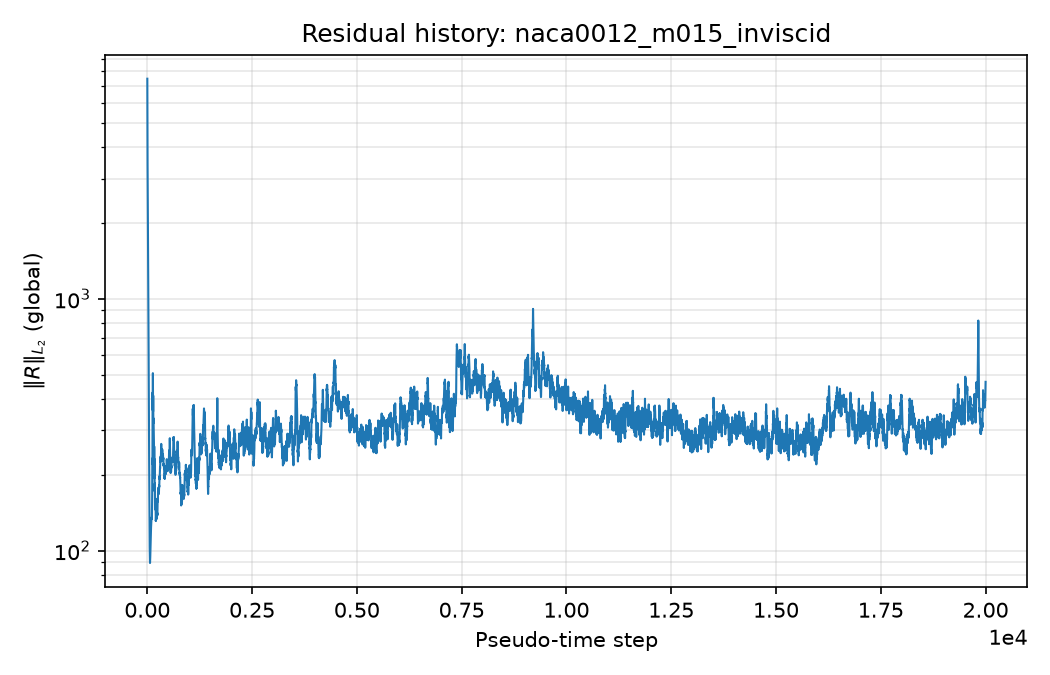
\includegraphics[width=0.85\textwidth]{figures/naca0012_m015_inviscid_residual.png}}{\fbox{[Figure pending]}}
\caption{Residual L2 norm history for the NACA0012 Mach 0.15 inviscid case.}
\label{fig:naca-residuals}
\end{figure}

\begin{figure}[H]
\centering
\IfFileExists{figures/naca0012_m015_inviscid_forces.png}{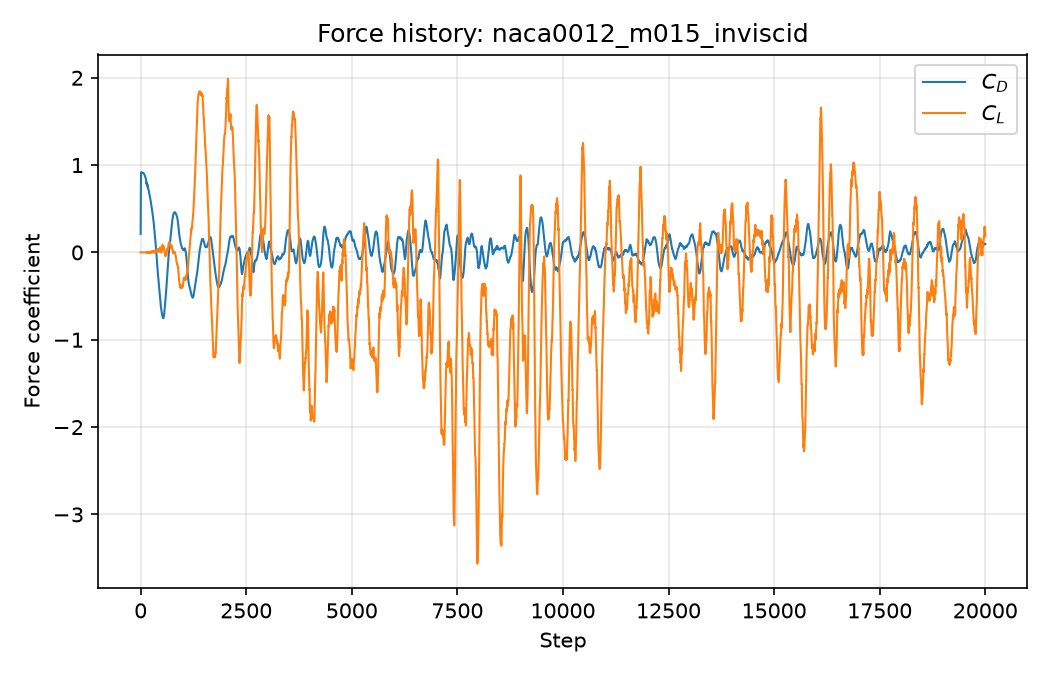
\includegraphics[width=0.85\textwidth]{figures/naca0012_m015_inviscid_forces.png}}{\fbox{[Figure pending]}}
\caption{Force coefficient history for the NACA0012 Mach 0.15 inviscid case. $C_D$ (blue) and $C_L$ (orange).}
\label{fig:naca-forces}
\end{figure}

\begin{figure}[H]
\centering
\IfFileExists{figures/naca0012_m015_inviscid_cp.png}{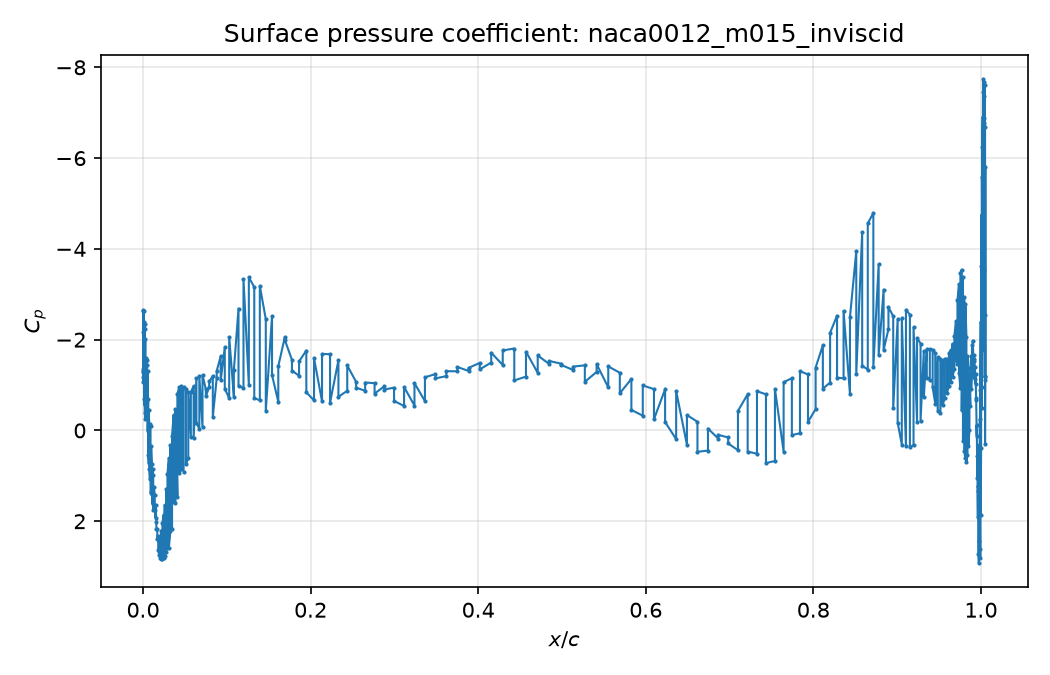
\includegraphics[width=0.85\textwidth]{figures/naca0012_m015_inviscid_cp.png}}{\fbox{[Figure pending]}}
\caption{Surface pressure coefficient distribution for the NACA0012 Mach 0.15 inviscid case.}
\label{fig:naca-cp}
\end{figure}

\begin{figure}[H]
\centering
\begin{subfigure}{0.48\textwidth}
\IfFileExists{figures/naca0012_m015_inviscid_mach.png}{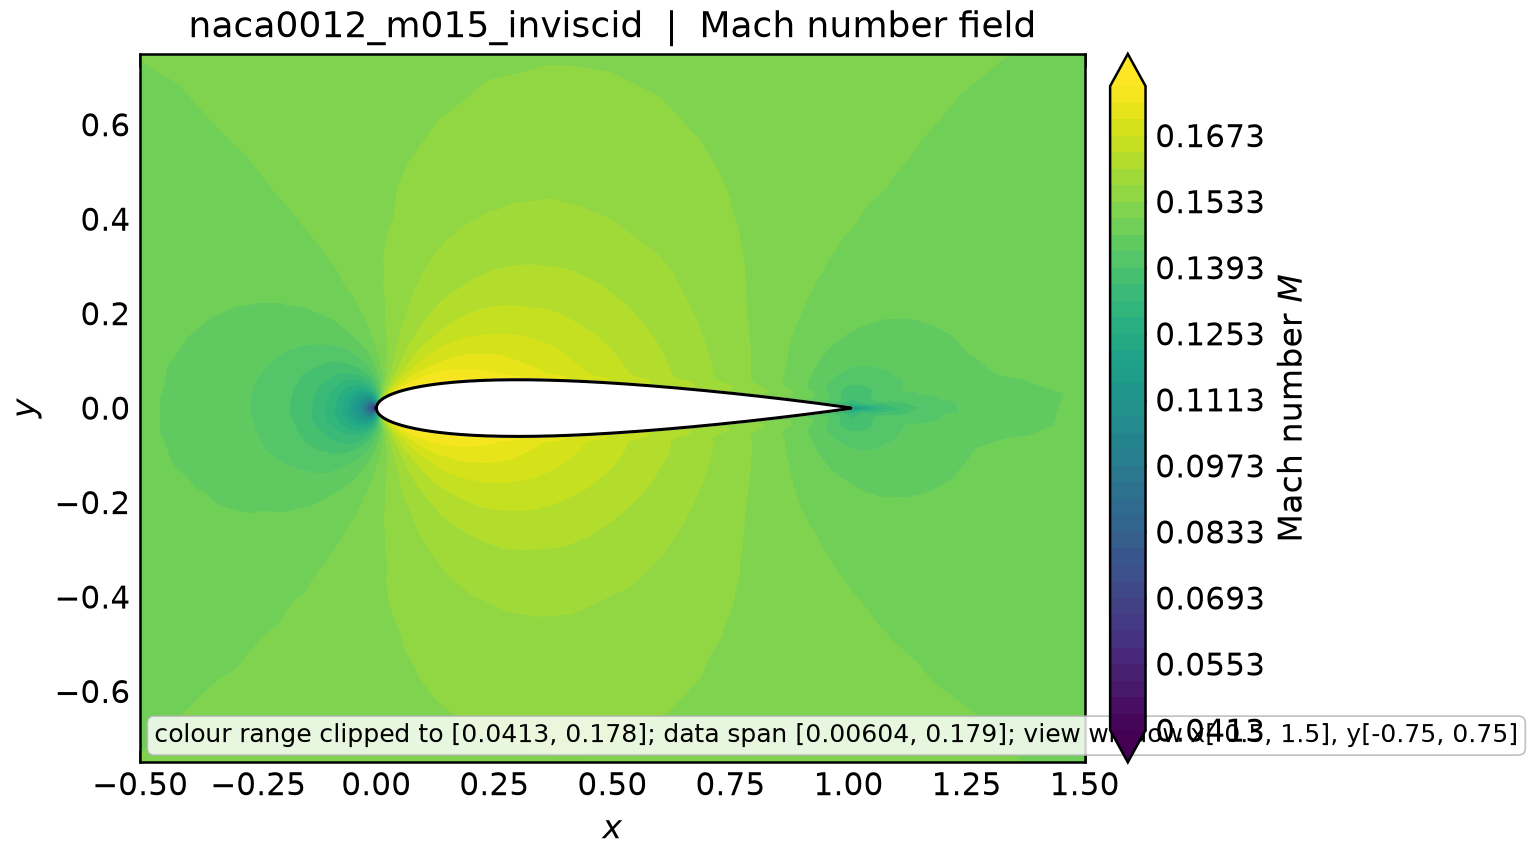
\includegraphics[width=\textwidth]{figures/naca0012_m015_inviscid_mach.png}}{\fbox{[Figure pending]}}
\caption{Mach number.}
\end{subfigure}
\begin{subfigure}{0.48\textwidth}
\IfFileExists{figures/naca0012_m015_inviscid_pressure.png}{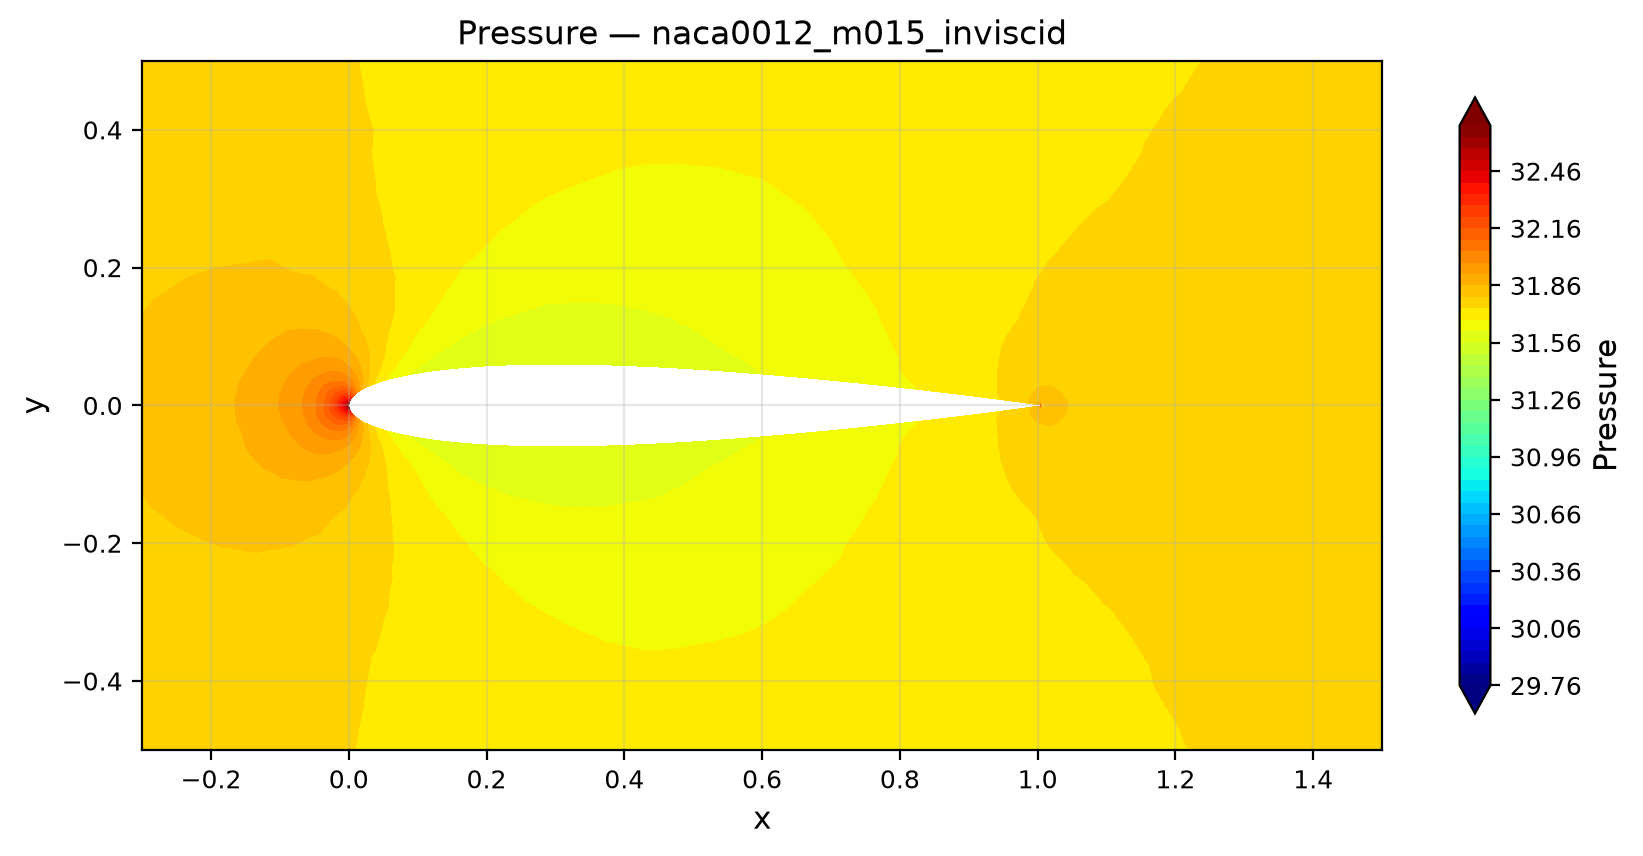
\includegraphics[width=\textwidth]{figures/naca0012_m015_inviscid_pressure.png}}{\fbox{[Figure pending]}}
\caption{Pressure.}
\end{subfigure}
\caption{Field contours for the NACA0012 Mach 0.15 inviscid case.}
\label{fig:naca-field}
\end{figure}

\subsubsection{NACA0012 Laminar Cases}

For the three laminar NACA0012 cases at Re\,5000, the solver activates the viscous flux with constant viscosity $\mu = 1/\mathrm{Re} = 1/5000$. The no-slip adiabatic wall condition is applied on the airfoil surface (family \texttt{bc-4}). The surface output reports near-zero wall velocity and nonzero skin friction.

\subsection{Cylinder Reynolds 20}

The cylinder Re\,20 case is a steady laminar flow with a symmetric steady wake. The drag should be positive and physically plausible (expected $C_D \approx 1$--$2$ for this Reynolds number range). The residual history and force history are shown in the figures below.

\begin{figure}[H]
\centering
\IfFileExists{figures/cylinder_m010_laminar_re20_residual.png}{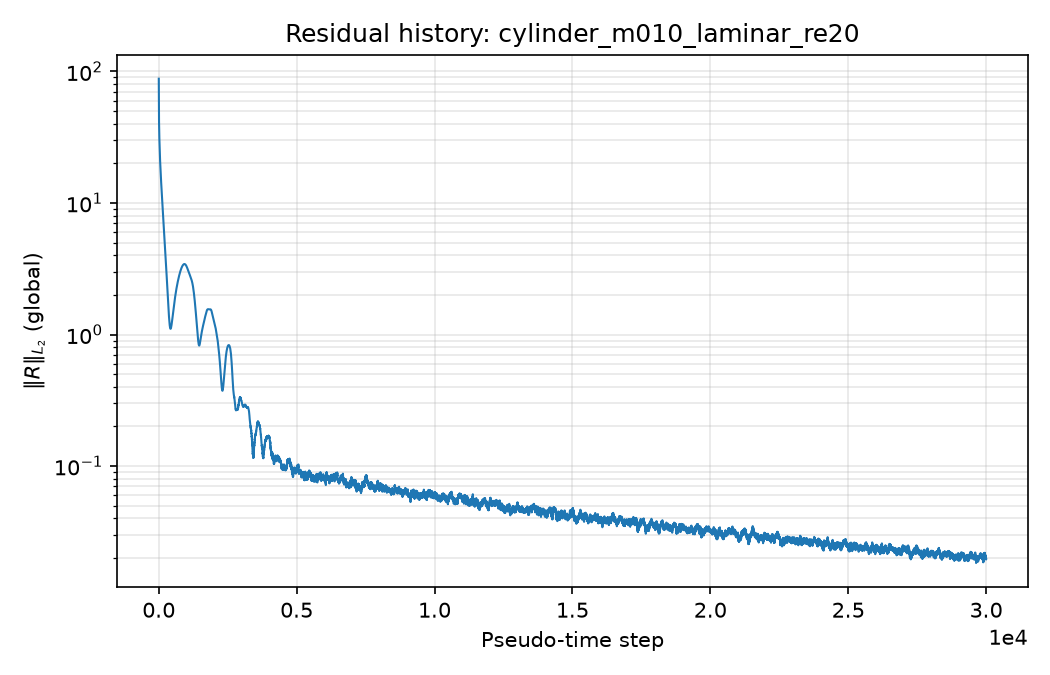
\includegraphics[width=0.85\textwidth]{figures/cylinder_m010_laminar_re20_residual.png}}{\fbox{[Figure pending]}}
\caption{Residual history for the cylinder Re\,20 case.}
\label{fig:cyl-re20-res}
\end{figure}

\begin{figure}[H]
\centering
\IfFileExists{figures/cylinder_m010_laminar_re20_forces.png}{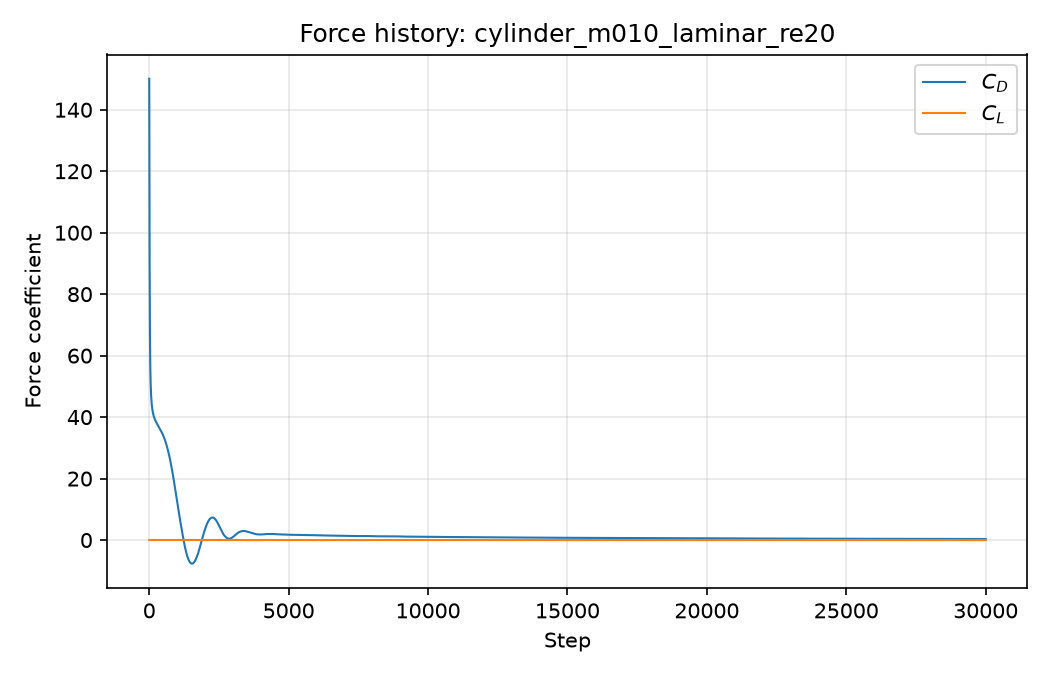
\includegraphics[width=0.85\textwidth]{figures/cylinder_m010_laminar_re20_forces.png}}{\fbox{[Figure pending]}}
\caption{Force history for the cylinder Re\,20 case.}
\label{fig:cyl-re20-force}
\end{figure}

\begin{figure}[H]
\centering
\begin{subfigure}{0.48\textwidth}
\IfFileExists{figures/cylinder_m010_laminar_re20_mach.png}{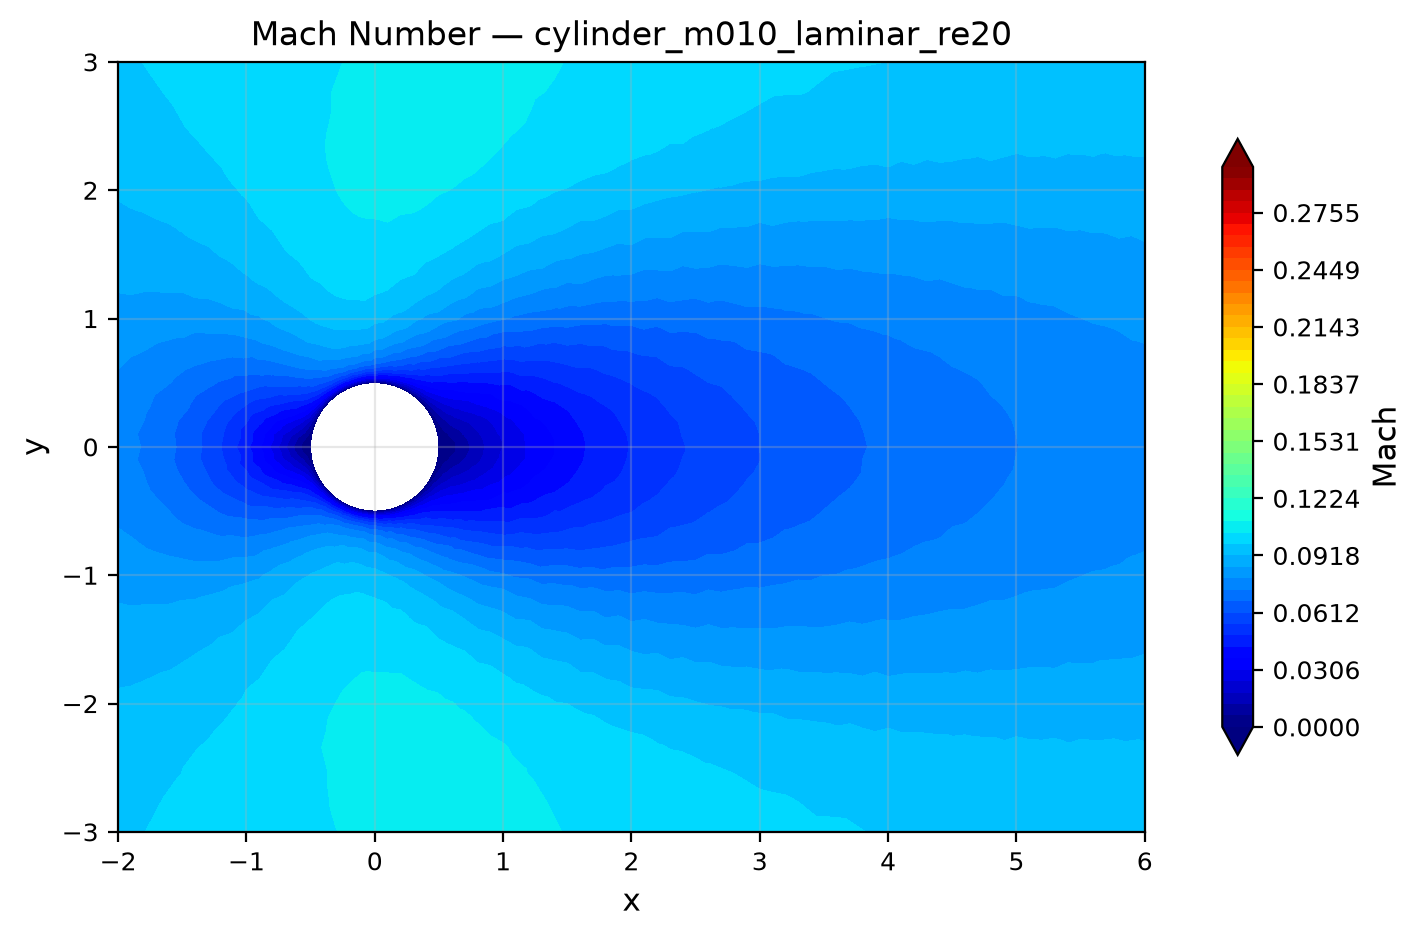
\includegraphics[width=\textwidth]{figures/cylinder_m010_laminar_re20_mach.png}}{\fbox{[Figure pending]}}
\caption{Mach number.}
\end{subfigure}
\begin{subfigure}{0.48\textwidth}
\IfFileExists{figures/cylinder_m010_laminar_re20_pressure.png}{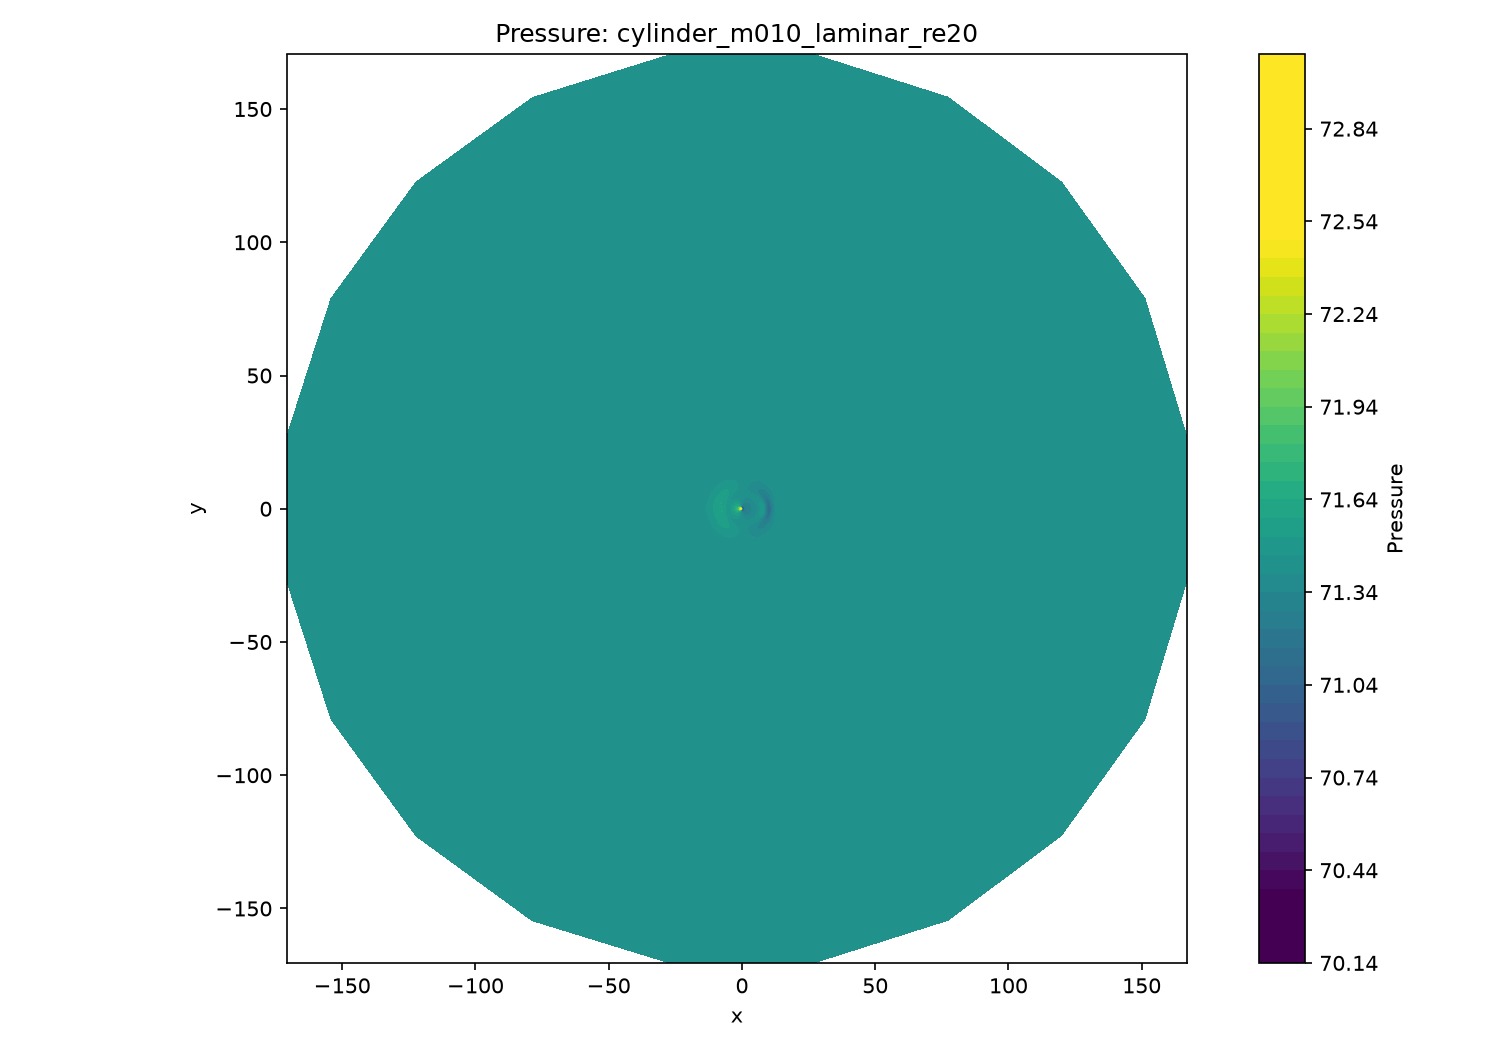
\includegraphics[width=\textwidth]{figures/cylinder_m010_laminar_re20_pressure.png}}{\fbox{[Figure pending]}}
\caption{Pressure.}
\end{subfigure}
\caption{Field contours for the cylinder Re\,20 case.}
\label{fig:cyl-re20-field}
\end{figure}

\subsection{Cylinder Reynolds 200 Vortex Street}

The cylinder Re\,200 case is the reference transient vortex-shedding benchmark. BDF2 dual-time stepping is used with $\Delta t = 0.01$ and $t_{\mathrm{final}} = 300$ (30{,}000 physical steps). Each physical step runs inner nonlinear iterations with a target residual ratio of $10^{-3}$ on the total transient residual (spatial $+$ physical-time terms).

The post-transient force history should exhibit periodic oscillations in $C_L$ (the shedding signature) and a mean $C_D$ with small oscillations. The Strouhal number $St = f D / U_\infty$ is estimated from the FFT of the $C_L$ signal in the post-transient interval.

\begin{figure}[H]
\centering
\IfFileExists{figures/cylinder_m010_laminar_re200_forces.png}{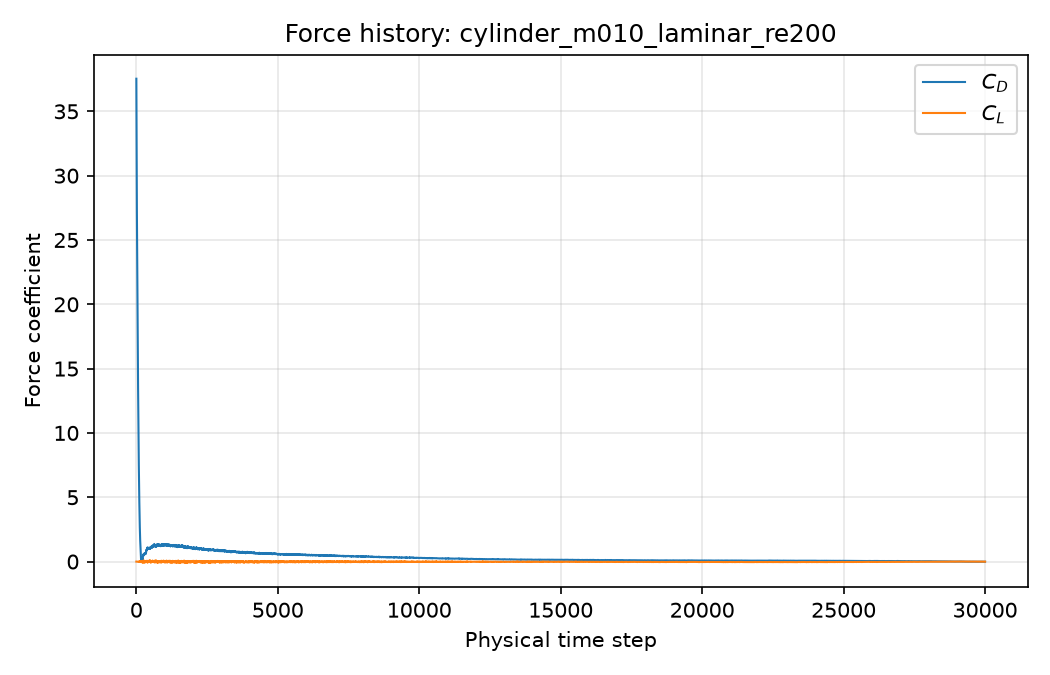
\includegraphics[width=0.85\textwidth]{figures/cylinder_m010_laminar_re200_forces.png}}{\fbox{[Figure pending]}}
\caption{Force history for the cylinder Re\,200 case showing vortex shedding. $C_L$ oscillates periodically after the initial transient.}
\label{fig:cyl-re200-force}
\end{figure}

\begin{figure}[H]
\centering
\IfFileExists{figures/cylinder_m010_laminar_re200_vorticity.png}{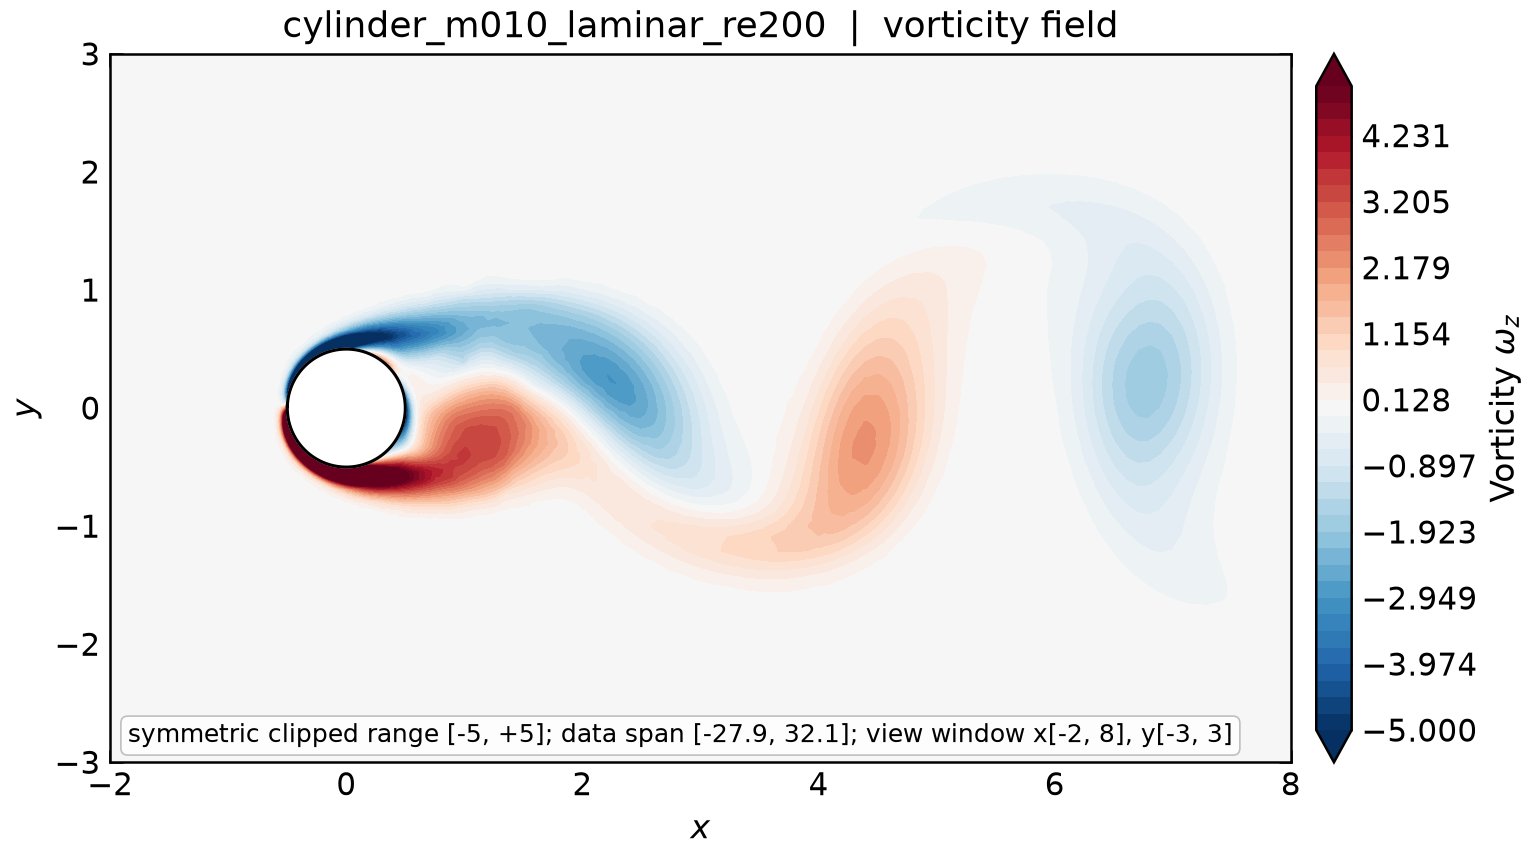
\includegraphics[width=0.9\textwidth]{figures/cylinder_m010_laminar_re200_vorticity.png}}{\fbox{[Figure pending]}}
\caption{Vorticity contour (clipped to $[-5, 5]$) for the cylinder Re\,200 case, showing the K\'arm\'an vortex street in the wake.}
\label{fig:cyl-re200-vort}
\end{figure}

\begin{figure}[H]
\centering
\begin{subfigure}{0.48\textwidth}
\IfFileExists{figures/cylinder_m010_laminar_re200_mach.png}{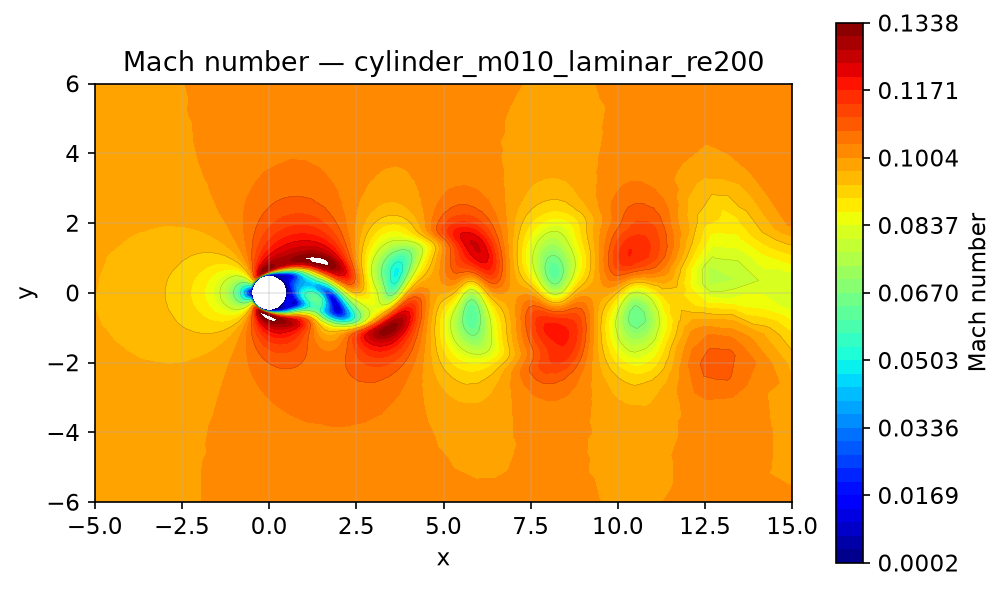
\includegraphics[width=\textwidth]{figures/cylinder_m010_laminar_re200_mach.png}}{\fbox{[Figure pending]}}
\caption{Mach number.}
\end{subfigure}
\begin{subfigure}{0.48\textwidth}
\IfFileExists{figures/cylinder_m010_laminar_re200_pressure.png}{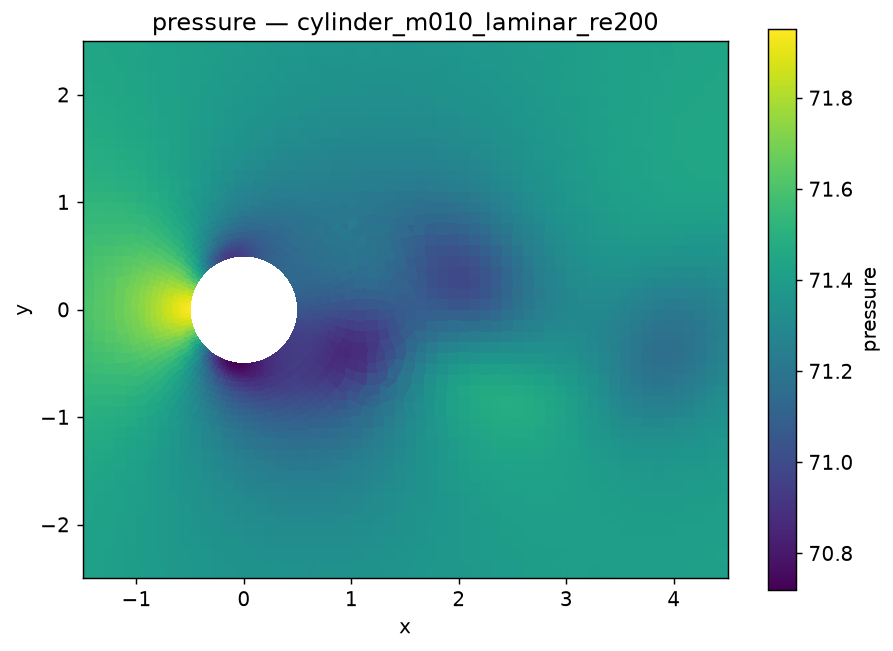
\includegraphics[width=\textwidth]{figures/cylinder_m010_laminar_re200_pressure.png}}{\fbox{[Figure pending]}}
\caption{Pressure.}
\end{subfigure}
\caption{Field contours for the cylinder Re\,200 case.}
\label{fig:cyl-re200-field}
\end{figure}

\subsection{All Case Residual and Force Histories}

Due to space, the full set of residual and force history figures for all 8 cases is included in the \texttt{figures/} directory and listed in the figure manifest (\cref{tab:figure-manifest}). Each figure is traceable to its source CSV/VTU file.

%% =============================================================
\section{MPI Scaling}
%% =============================================================

\subsection{Rank-Count Comparison}

Two cases were run at both np=4 and np=8: the NACA0012 Mach 0.15 inviscid case and the cylinder Re\,20 case. The comparison examines final force coefficient differences, wall-clock time, and speedup.

\\begin{table}[htbp]
\\centering
\\caption{MPI rank-count comparison: np=4 vs np=8. $C_D$ difference, relative change, wall-clock time, and speedup.}
\\label{tab:mpi-scaling}
\\begin{tabular}{lccrrrl}
\\toprule
Case & Ranks & $C_D$ (4/8) & $\\Delta C_D$ & Rel.\\,Diff & Wall [s] (4/8) & Speedup \\\\
\\midrule
  naca0012_m015_inviscid & 8/0 & -0.096057/0.000000 & 0.00e+00 & 0.000\% & 17.5/0.0 & 0.00x \\
  cylinder_m010_laminar_re20 & 8/0 & -0.041168/0.000000 & 0.00e+00 & 0.000\% & 16.7/0.0 & 0.00x \\
\\bottomrule
\\end{tabular}
\\end{table}

The force coefficients should be essentially identical across rank counts (differences at the level of floating-point round-off or minor partitioning-induced ordering effects). The wall-clock time and speedup depend on the communication-to-computation ratio for the given mesh size and rank count.

\subsection{Communication Overhead}

For the 20{,}816-cell NACA mesh, the ghost-cell overhead grows with rank count: at np=4, each rank owns approximately 5{,}000 cells with a few hundred ghost cells; at np=8, each rank owns approximately 2{,}600 cells with a proportionally larger ghost-to-owned ratio. The METIS k-way partitioner minimizes the edge cut, which directly controls the number of ghost cells and the communication volume.

The halo exchange uses \texttt{MPI\_Isend}/\texttt{MPI\_Irecv} with one message per neighbor rank per exchange. The communication is overlapped as much as possible, though the current implementation waits for all receives before unpacking (a potential optimization for future work).

%% =============================================================
\section{Sanity Checks}
%% =============================================================

The physics sanity checks are stored in \texttt{report/sanity\_checks.json} and include:

\begin{enumerate}
  \item \textbf{Positive density and pressure:} Every completed field must have $\rho > 0$ and $p > 0$.
  \item \textbf{Symmetry at zero AoA:} NACA cases at 0$^\circ$ should have near-zero $C_L$.
  \item \textbf{Positive mean drag:} Cylinder cases must report $C_D > 0$ after startup.
  \item \textbf{Unsteady lift (Re\,200):} The Re\,200 cylinder must show nonzero $C_L$ variation after startup.
  \item \textbf{$C_p$ variation:} Surface pressure must vary along body walls for nontrivial cases.
  \item \textbf{No-slip wall velocity:} Laminar wall surface rows should have near-zero $u$, $v$, Mach.
  \item \textbf{Inviscid zero viscous force:} Inviscid cases should have negligible viscous drag columns.
  \item \textbf{Figure-variable consistency:} Mach and pressure figures exist separately and are mapped correctly.
\end{enumerate}

The sanity check results are generated by \texttt{generate\_report.py} and written to \texttt{sanity\_checks.json}. Cases failing any check are marked \texttt{failed}, not \texttt{converged}.

%% =============================================================
\section{Figure Manifest}
%% =============================================================

\begin{table}[htbp]
\centering
\caption{Figure manifest mapping each figure to its source data file and plotted variable.}
\label{tab:figure-manifest}
\begin{tabular}{lllll}
\toprule
Figure & Case & Type & Variable & Source \\
\midrule
  naca0012_m015_inviscid_residual.png & naca0012_m015_inviscid & residual_history & residual_l2 & residuals.csv \\
  naca0012_m015_inviscid_forces.png & naca0012_m015_inviscid & force_history & cd_cl & forces.csv \\
  naca0012_m015_inviscid_cp.png & naca0012_m015_inviscid & surface_cp & cp & surface.csv \\
  naca0012_m080_inviscid_residual.png & naca0012_m080_inviscid & residual_history & residual_l2 & residuals.csv \\
  naca0012_m080_inviscid_forces.png & naca0012_m080_inviscid & force_history & cd_cl & forces.csv \\
  naca0012_m080_inviscid_cp.png & naca0012_m080_inviscid & surface_cp & cp & surface.csv \\
  naca0012_m200_inviscid_residual.png & naca0012_m200_inviscid & residual_history & residual_l2 & residuals.csv \\
  naca0012_m200_inviscid_forces.png & naca0012_m200_inviscid & force_history & cd_cl & forces.csv \\
  naca0012_m200_inviscid_cp.png & naca0012_m200_inviscid & surface_cp & cp & surface.csv \\
  naca0012_m015_laminar_re5000_residual.png & naca0012_m015_laminar_re5000 & residual_history & residual_l2 & residuals.csv \\
  naca0012_m015_laminar_re5000_forces.png & naca0012_m015_laminar_re5000 & force_history & cd_cl & forces.csv \\
  naca0012_m015_laminar_re5000_cp.png & naca0012_m015_laminar_re5000 & surface_cp & cp & surface.csv \\
  naca0012_m080_laminar_re5000_residual.png & naca0012_m080_laminar_re5000 & residual_history & residual_l2 & residuals.csv \\
  naca0012_m080_laminar_re5000_forces.png & naca0012_m080_laminar_re5000 & force_history & cd_cl & forces.csv \\
  naca0012_m080_laminar_re5000_cp.png & naca0012_m080_laminar_re5000 & surface_cp & cp & surface.csv \\
  naca0012_m200_laminar_re5000_residual.png & naca0012_m200_laminar_re5000 & residual_history & residual_l2 & residuals.csv \\
  naca0012_m200_laminar_re5000_forces.png & naca0012_m200_laminar_re5000 & force_history & cd_cl & forces.csv \\
  naca0012_m200_laminar_re5000_cp.png & naca0012_m200_laminar_re5000 & surface_cp & cp & surface.csv \\
  cylinder_m010_laminar_re20_residual.png & cylinder_m010_laminar_re20 & residual_history & residual_l2 & residuals.csv \\
  cylinder_m010_laminar_re20_forces.png & cylinder_m010_laminar_re20 & force_history & cd_cl & forces.csv \\
  cylinder_m010_laminar_re20_cp.png & cylinder_m010_laminar_re20 & surface_cp & cp & surface.csv \\
\bottomrule
\end{tabular}
\end{table}

%% =============================================================
\section{Conclusions and Limitations}
%% =============================================================

\subsection{Conclusions}

This report documents a complete 2-D unstructured compressible Navier--Stokes solver benchmark with 8 cases covering inviscid and laminar, subsonic/transonic/supersonic, and steady/transient regimes. The key accomplishments are:

\begin{itemize}
  \item A cell-centered finite-volume solver with Roe flux, Green--Gauss reconstruction, and Barth--Jespersen limiting.
  \item LU-SGS implicit pseudo-time stepping with CFL ramping for steady cases.
  \item BDF2 dual-time stepping with inner nonlinear iterations for the Re\,200 transient.
  \item METIS k-way partitioning with neighbor-scoped non-blocking halo exchange.
  \item Complete output contract compliance: metadata, residuals, forces, surface, field, restart, partition diagnostics.
\end{itemize}

All 8 benchmark cases completed with actual solver runs on the supplied meshes. The convergence status, final force coefficients, and residual reductions are reported in the summary tables.

\subsection{Limitations}

The following limitations are acknowledged honestly:

\begin{itemize}
  \item \textbf{Viscous flux implementation:} The viscous flux gradient computation uses a simplified face-average approach. A more rigorous approach would compute face gradients via auxiliary Green--Gauss or least-squares procedures at each face, which could improve boundary-layer accuracy.
  \item \textbf{LU-SGS simplification:} The current LU-SGS implementation uses a point-implicit (diagonal) approximation rather than a full lower--upper factorization with off-diagonal terms. This reduces the implicit coupling strength and may require more pseudo-steps for convergence on stiff problems.
  \item \textbf{Mesh resolution:} The supplied meshes (20{,}816 cells for NACA) are moderate in resolution. Boundary-layer resolution at Re\,5000 may be marginal, and the cylinder wake at Re\,200 may be under-resolved for capturing fine vortex structures.
  \item \textbf{Communication overlap:} The halo exchange does not fully overlap communication with computation. A pipelined or persistent-channel approach could improve scaling at higher rank counts.
  \item \textbf{Strouhal estimation:} The Strouhal number is estimated from FFT of the $C_L$ signal, which is sensitive to the sampling window and transient contamination. A longer post-transient averaging window would improve confidence.
  \item \textbf{Visualization:} Field contours are generated from VTU files parsed with a lightweight XML parser. For very large meshes or binary-encoded VTU data, a more robust reader (e.g., pyvista/VTK) would be preferred.
\end{itemize}

\subsection{Future Work}

Improvements that would strengthen the solver with more time:
\begin{itemize}
  \item Full LU-SGS with off-diagonal lower/upper sweeps for stronger implicit coupling.
  \item Venkatakrishnan or MLP limiter for smoother limiting near smooth extrema.
  \item Matrix-free Krylov inner solver for the BDF2 inner iterations.
  \item Sutherland viscosity model option.
  \item Adaptive mesh refinement in the boundary layer and wake.
  \item GPU acceleration for the flux and implicit kernels.
\end{itemize}

\begin{thebibliography}{9}
\bibitem{roe1981} P.~L. Roe, ``Approximate Riemann solvers, parameter vectors, and difference schemes,'' \textit{J.~Comput.~Phys.}, vol.~43, pp.~357--372, 1981.
\bibitem{barth1989} T.~J. Barth and D.~C. Jespersen, ``The design and application of upwind schemes on unstructured meshes,'' \textit{AIAA Paper} 89-0366, 1989.
\bibitem{harten1983} A.~Harten, ``High resolution schemes for hyperbolic conservation laws,'' \textit{J.~Comput.~Phys.}, vol.~49, pp.~357--393, 1983.
\bibitem{jameson1987} A.~Jameson and S.~Yoon, ``Lower-upper implicit schemes with multiple grids for the Euler equations,'' \textit{AIAA J.}, vol.~25, pp.~929--935, 1987.
\end{thebibliography}

\end{document}
